\chapter{Analisis Masalah dan Rancangan Solusi}

Tujuan utama penulisan bab ini adalah untuk menguraikan rencana penyelesaian masalah implementasi sistem \textit{remote deployment} pada lingkungan IoT. Bagian ini memaparkan proses analisis masalah hingga menjadi solusi.


\section{Analisis}

% Sistem tiket yang dibahas pada penelitian ini merupakan sistem dengan karakteristik sebagaimana dibahas pada lampiran \ref{apx:analisis-kebutuhan}.

\section{Analisis Masalah}

Penjualan tiket acara dengan tingkat peminat serupa dengan penjualan tiket Taylor Swift dan Coldplay tentu akan terjadi lagi di masa mendatang. Meskipun begitu, tidak semua penyedia layanan terbiasa menangani beban pada skala ini. Kebanyakan penyedia layanan menggunakan solusi antrean virtual yang membatasi jumlah pengguna yang mengakses situs secara bersamaan. Pendekatan ini memang membantu meringankan beban sistem dan menjaga stabilitas. Meskipun begitu, banyak pengguna yang harus menunggu lama untuk bisa mengakses platform.

Di sisi lain, belum banyak studi yang membahas skalabilitas sistem dengan kasus seperti ini. \cite{microservicesEventDriven} membahas desain arsitektur yang \textit{fault-tolerant} dan tidak membahas aspek skalabilitas. \cite{backendForTicketing} juga tidak membahas arsitektur sistem dari sisi skalabilitas. \cite{barua2024enhancingresiliencescalabilitytravel} membahas desain sistem pemesanan tiket pesawat dengan arsitektur \textit{microservice}. Pengoptimalan \textit{fault tolerance} dan \textit{load balancing} memungkinkan penggunaan sumber daya yang lebih optimal, sehingga \textit{throughput} meningkat. Meskipun begitu, penelitian tersebut tidak membahas pengoptimalan pada pola akses basis data. Berdasarkan pertimbangan di atas, diperlukan desain arsitektur yang optimal dan mampu menangani beban seperti ini. Solusi ini tidak serta merta mengganti solusi antrean virtual. Dengan adanya arsitektur yang optimal, jumlah pengguna yang bisa dilayani dalam satu waktu dapat meningkat dan proses penjualan menjadi lebih cepat tanpa kendala.

Beban sistem tiket dapat dibagi menjadi dua: permintaan baca ketersediaan tiket dan proses pemesanan tiket. Sebagaimana digambarkan pada figur \ref{fig:event-rm} dan \ref{fig:ticket-storage}, kueri ketersediaan harus mengagregasi beberapa entitas yang saling berhubungan. Operasi ini berat apabila dilakukan dengan jumlah yang sangat banyak, seperti saat banyak pengguna ingin membeli tiket dalam waktu yang bersamaan. Hasil kueri ini tidak dapat di-\textit{cache} karena data selalu berubah saat penjualan sehingga data akan langsung \textit{stale}. Selain itu, akan ada banyak pengguna yang ingin memesan tiket secara bersamaan, sehingga terjadi \textit{write contention}. Skema \textit{locking} dan \textit{flow control} diperlukan agar percobaan pembelian tiket yang sama dapat berkurang Selain itu, \textit{throughput} pemrosesan pesanan juga perlu ditingkatkan.

% \subsection{Alternatif Solusi}
\label{sec:analisis-solusi}

Berdasarkan analisis permasalahan pada bagian \ref{sec:analisis-permasalahan} serta studi literatur, Terdapat tiga alternatif solusi dalam pembuatan PERISAI. yaitu membuat arsitektur berbasis Kubernetes, arsitektur berbasis \textit{apache zookeper}, serta membuat arsitektur dengan mengikuti referensi yang sudah ada.

\subsubsection{Membuat sistem berbasis Kubernetes}
Kubernetes, sebagai layanan orkestrasi kontainer yang kuat, menawarkan mekanisme otomatisasi \textit{deployment}, skalabilitas, dan manajemen aplikasi yang sangat cocok untuk lingkungan \textit{cloud} dan terdistribusi. Dalam konteks IoT, Kubernetes bisa dimanfaatkan untuk mengelola dan mengorkestrasi aplikasi berbasis kontainer pada lingkungan IoT ataupun pada \textit{cloud}. Kubernetes mendukung model \textit{microservices} yang fleksibel dan resilien serta memiliki banyak kelebihan yaitu meliputi kemampuan autoscaling, pemulihan otomatis dari kegagalan, dan manajemen beban kerja yang efisien. Kubernetes dapat memanfaatkan \textit{affinity selector} untuk melakukan \textit{targeted deployment}, sehingga proses \textit{deployment} dapat diberikan kepada perangkat yang memerlukan \textit{deployment} saja. Namun, Kubernetes juga memiliki kekurangan yaitu membutuhkan sumber daya yang relatif tinggi, yang mungkin tidak ideal untuk perangkat IoT dengan keterbatasan sumber daya. Namun, hal ini dapat diatasi dengan distribusi Kubernetes yang khusus dibuat untuk lingkungan IoT yaitu microk8s, K3s, serta KubeEdge. Dari ketiga solusi ini, distribusi K3s dapat dijalankan pada perangkat yang hanya memiliki RAM 900mb tanpa ada masalah. Selain itu kemudahan dalam penggunaan dan supportnya untuk seluruh arsitektur membuat K3s menjadi pilihan yang digunakan untuk tugas akhir ini. Perbandingan ketiga distribusi dapat dilihat pada lampiran \ref{tab:perbandingan-distribusi-kubernetes}.

\subsubsection{Membuat sistem berbasis \textit{Apache ZooKeper}}
Apache ZooKeeper menyediakan layanan koordinasi terdistribusi yang sangat diperlukan pada lingkungan aplikasi terdistribusi. Dalam konteks sistem \textit{remote deployment} pada lingkungan IoT, ZooKeeper dapat dimanfaatkan untuk mengelola konfigurasi dan melakukan sinkronisasi diantara komponen sistem terutama pada lingkungan terdistribusi. Kelebihan menggunakan ZooKeeper antara lain konsistensi data yang tinggi dan model pemrograman yang relatif sederhana. Kekurangannya, ZooKeeper tidak secara langsung mendukung kasus \textit{deployment} aplikasi karena hanya berfokus pada masalah konfigurasi, Selain itu zookeper juga membutuhkan \textit{resource} yang sangat besar sehingga bisa menjadi \textit{bottleneck} jika tidak dirancang dengan hati-hati, terutama dalam lingkungan dengan jumlah perangkat yang sangat besar. Zookeper juga tidak Oleh karena itu, diperlukan adanya penyesuaian dan adopsi agar menjadi kompatibel dan tidak menjadi \textit{bottleneck}.

\subsubsection{Membuat sistem berbasis LEONORE dan DIANE}
Mengembangkan sistem provisioning skala besar berbasis LEONORE dan DIANE sudah menyelesaikan beberapa masalah yang telah disebutkan. Namun kekurangannya ialah, desain menjadi tidak fleksibel, sulit untuk dikustomisasi, serta terdapat resiko keamanan jika tidak mengimplementasikan dengan benar. Selain itu proses implementasi membutuhkan waktu yang lama. Proses pengujian yang sulit pun menjadi salah satu tantangan dalam mengimplementasikan metode ini.

\pagebreak

Berdasarkan ketiga alternatif solusi yang telah dijelaskan, Dipilihlah kubernetes sebagai dasar dari PERISAI. Alasan pemilihan kubernetes karena menjawab permasalahan yang telah dijelaskan pada bagian \ref{sec:analisis-permasalahan} khususnya \textit{targeted deployment}.Perbandingan ketiga alternatif solusi dapat dilihat pada tabel \ref{tab:perbandingan-analisis-solusi}.

\bgroup
\begin{table}[ht]
  \def\arraystretch{1.3}
  \caption{Perbandingan Ketiga Alternatif Solusi}
  \label{tab:perbandingan-analisis-solusi}
  \centering
  \begin{tabular}{|p{2cm}|p{2cm}|p{2cm}|p{1.8cm}|p{1.7cm}|p{1.7cm}|}
    \hline
    Solusi           & Berjalan di berbagai perangkat                            & Melakukan \textit{targeted deployment} & Berjalan pada perangkat dengan sumber daya terbatas & Mengatur banyak perangkat & Waktu pembuatan sistem \\
    \hline
    Kubernetes       & Ya, seluruh perangkat yang dapat melakukan kontainerisasi & Ya                                     & Ya dengan K3s                                       & Ya                        & Cepat                  \\
    \hline
    Zookeper         & Ya, seluruh perangkat yang memiliki java                  & Tidak                                  & Tidak                                               & Ya                        & Cepat                  \\
    \hline
    LEONORE \& DIANE & Tidak                                                     & Tidak                                  & Mungkin                                             & Ya                        & Lama                   \\
    \hline
  \end{tabular}
\end{table}
\egroup

% \subsection{Analisis Kebutuhan Sistem}
\label{sec:analisis-kebutuhan-sistem}

Berdasarkan bagian \ref{sec:analisis-solusi}, Kubernetes menjadi pilihan solusi yang digunakan karena memiliki berbagai kelebihan dibandingkan dengan pendekatan lain terutama dalam hal \textit{targeted deployment}. Kubernetes, sebagai sistem orkestrasi kontainer yang matang dan luas digunakan, menawarkan fitur dan kemampuan yang cocok untuk mengatasi tantangan yang dihadapi dalam lingkungan IoT yang heterogen dan terdistribusi terutama dalam masalah skalabilitas, \textit{ready to use}, serta memakan waktu yang minimal sehingga solusi ini merupakan solusi paling \textit{feasible} yang dapat diimplementasikan.

PERISAI akan menggunakan kubernetes sebagai sistem orkestrasi dalam mengatur banyak perangkat. Namun, sebelum membuat arsitektur PERISAI, perlu dilakukan analisis kebutuhan untuk sistem yang diperlukan. PERISAI akan digunakan pada skala besar sehingga perlu adanya sebuah organisasi yang bertanggung jawab atas seluruh perangkat yang dimiliki. Selain itu, untuk melakukan manajemen perangkat pasti dibutuhkan satu atau lebih \textit{user} yang dapat melakukan proses manajemen perangkat ataupun \textit{remote deployment}. PERISAI juga harrus dapat mengelompkan satu atau lebih perangkat untuk memudahkan proses \textit{deployment}. Proses \textit{deployment} dapat dilakukan untuk satu perangkat atau lebih serta melakukan \textit{deployment} kepada beberapa grup yang telah dikelompokan. Berangkat dari permasalahan tersebut, akan diuraikan kebutuhan sistem yang terbagi menjadi kebutuhan fungsional dan non-fungsional.

\subsubsection{Deskripsi sistem}
Sistem yang dibuat merupakan sebuah sistem yang dapat melakukan \textit{remote deployment} ke perangkat yang terhubung ataupun ke sebagian perangkat yang diinginkan. Sistem memiliki dua komponen utama yaitu \textit{dashboard} sebagai \textit{frontend} serta API sebagai \textit{backend}. Komponen \textit{backend} ini memiliki dua modul eksternal dan satu modul internal. Kubernetes dan \textit{database} sebagai modul eksternal serta server sebagai penghubung modul eksternal dengan modul internal. Modul Kubernetes terhubung ke kluster yang diinginkan untuk melakukan proses \textit{remote deployment} ke masing-masing perangkat yang terhubung. Ilustrasi secara kasar dapat dilihat pada gambar \ref{fig:gambaran-umum-arsitektur}.

\begin{figure}[ht]
  \centering
  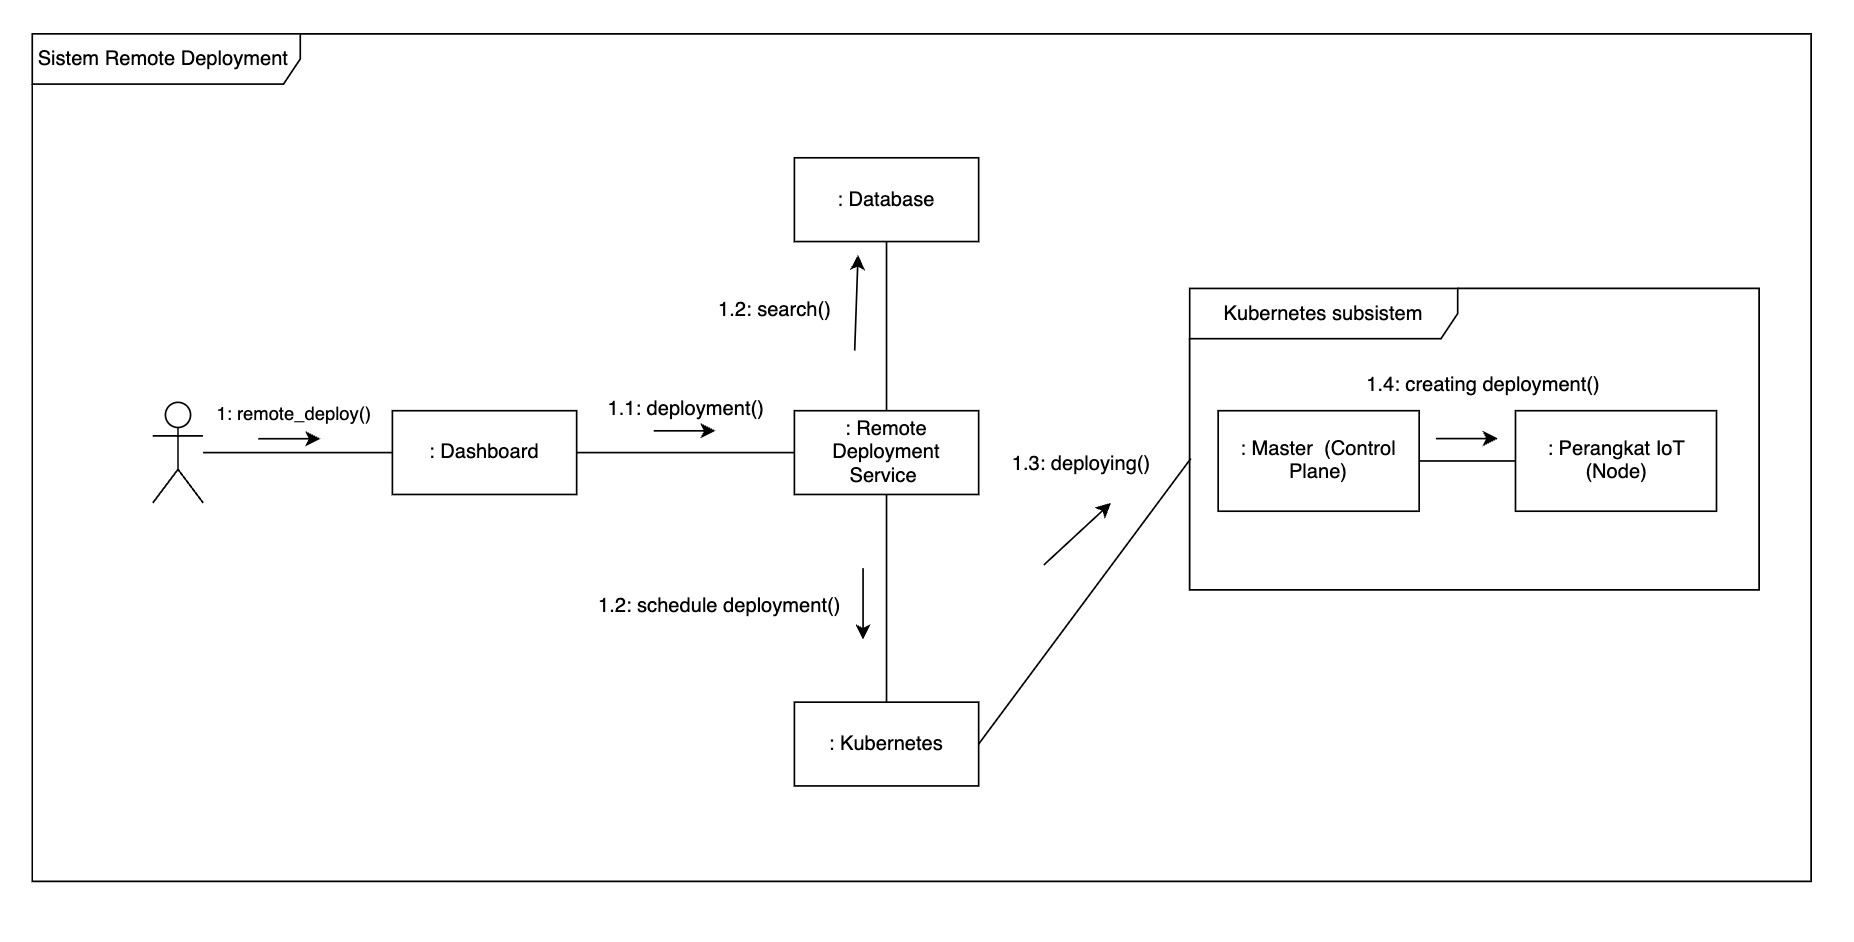
\includegraphics[width=1\textwidth]{resources/chapter-3/gambaran-umum-arsitektur-updated.jpg}
  \caption{Gambaran Umum Arsitektur PERISAI}
  \label{fig:gambaran-umum-arsitektur}
\end{figure}

\pagebreak
\subsubsection{Karakteristik Pengguna}
Berdasarkan hasil analisis, terdapat dua pengguna pada sistem ini, yaitu pengguna dan administrator. Penjelasan lebih detail dapat dilihat pada tabel \ref{tab:karakteristik-pengguna}.

\bgroup
\begin{table}[ht]
  \def\arraystretch{1.7}
  \caption{Karakteristik Pengguna}
  \label{tab:karakteristik-pengguna}
  \centering
  \begin{tabular}{|p{2cm}|p{8cm}|}
    \hline
    Kategori Pengguna & Hak akses                                                                                                                                                                                                                                                                           \\
    \hline
    \textit{User}     & \textit{User} dapat melakukan login, registrasi, melihat \textit{user} lain di satu perusahaan, melakukan manajemen perangkat, melakukan manajemen groups, melakukan manajemen \textit{deployment}, melakukan \textit{remote deployment}, serta melihat riwayat \textit{deployment} \\
    \hline
    Admin             & Admin dapat melakukan manajemen perusahaan, manajemen user, serta seluruh kegiatan yang user dapat lakukan                                                                                                                                                                          \\
    \hline
  \end{tabular}
\end{table}
\egroup

\subsubsection{Kebutuhan Fungsional}
Sistem memiliki beberapa kebutuhan fungsional yang dipetakan dalam bentuk tabel yang dapat dilihat pada lampiran \ref{tab:kebutuhan-fungsional}. Semua kebutuhan fungsional memiliki ID yang diawali dengan huruf F lalu diikuti dengan dua angka.



\subsubsection{Kebutuhan Non-Fungsional}
Sistem memiliki 2 parameter kebutuhan non-fungsional yang dapat dilihat pada tabel \ref{tab:kebutuhan-non-fungsional}. Semua kebutuhan non-fungsional memiliki awalan ID NF lalu diikuti oleh dua angka.

\bgroup
\begin{table}[ht]
  \def\arraystretch{1.7}
  \caption{Kebutuhan Non-Fungsional}
  \label{tab:kebutuhan-non-fungsional}
  \centering
  \begin{tabular}{|c|p{3cm}|p{8cm}|}
    \hline
    ID   & Parameter            & Kebutuhan                                                                                                                                                                                                                          \\
    \hline
    NF01 & \textit{Security}    & Sistem menjamin keamanan dari \textit{service} dengan cara menyediakan validasi pada \textit{middleware} serta setiap \textit{request} dapat terhindar dari serangan. Hanya \textit{user} yang terautentikasi yang bisa mengakses. \\
    \hline
    NF02 & \textit{Portability} & Sistem dapat diakses dimana saja melalui perangkat laptop.                                                                                                                                                                         \\
    \hline
  \end{tabular}
\end{table}
\egroup

\subsubsection{Model \textit{Use case}}
\label{subsec:model-usecase}
Dari beberapa kebutuhan fungsional serta karakteristik pengguna, dapat dibuat \textit{use case} yang mengelompokkan serta menggambarkan relasi antara aktor dan aksi yang dapat dilakukan. \textit{Use case} memiliki identifikasi yang berawalan dengan UC diikuti oleh dua angka. \textit{Use case} dapat dilihat secara detail pada lampiran \ref{tab:penjelasan-usecase-diagram}.

Dari pemetaan \textit{use case} pada lampiran \ref{tab:penjelasan-usecase-diagram}, dapat dibuat sebuah diagram yang menghubungkan relasi antara aktor dengan \textit{use case}-nya. Relasi  aktor dengan kapabilitas fungsional sistem dapat dilihat pada diagram use case di Gambar \ref{fig:usecase-diagram}.

\begin{figure}[ht]
  \centering
  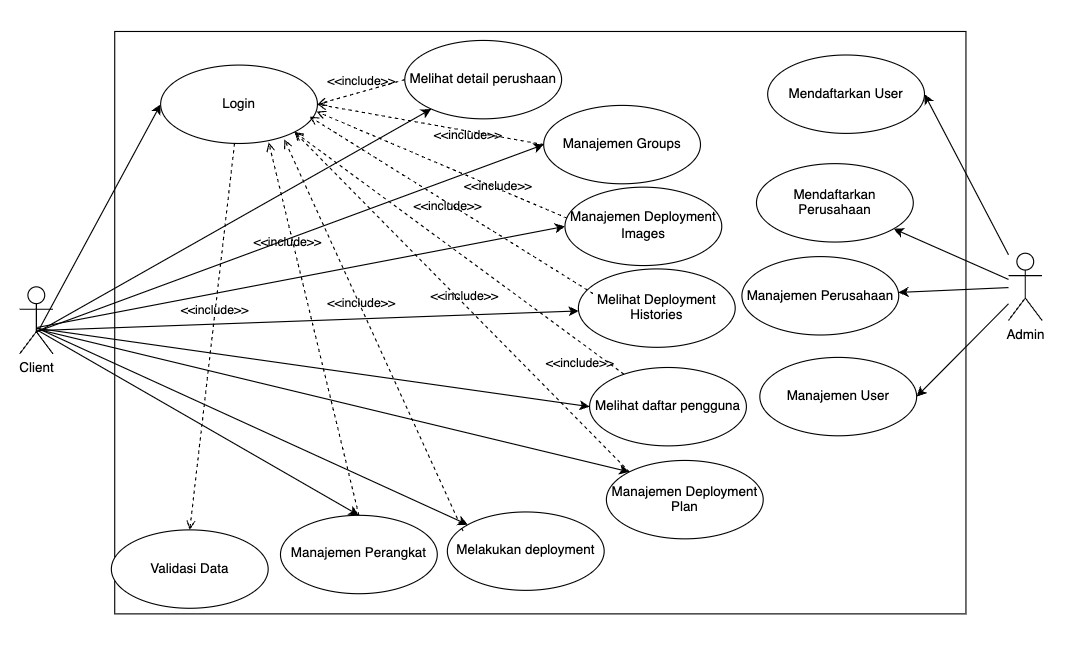
\includegraphics[width=1\textwidth]{resources/chapter-3/usecase-diagram.jpg}
  \caption{Usecase Diagram}
  \label{fig:usecase-diagram}
\end{figure}

\pagebreak


\section{Rancangan}

% Seperti yang telah dijelaskan pada gambar \ref{fig:gambaran-umum-arsitektur}, PERISAI memiliki dua komponen utama yaitu \textit{dashboard} dan \textit{service}. \textit{Dashboard} memiliki dua modul, yaitu modul untuk menampilkan halaman-halaman yang bersesuaian dan modul untuk melakukan koneksi dengan \textit{service}.

\textit{Service} memiliki tiga modul, yaitu server, \textit{database}, serta Kubernetes. Server menjadi pusat kontrol dari \textit{request} yang dikirimkan melalui \textit{dashboard}. Masing-masing perangkat diatur oleh modul Kubernetes yang telah memiliki sistem kluster terpisah. Penjelasan arsitektur secara detail dijelaskan pada dua subbab, yaitu arsitektur struktural serta arsitektur \textit{behavioural}.

\subsection{Rancangan Struktural}
\label{subsec:arsitektur-struktural}

Arsitektur struktural yang digunakan ialah \textit{package diagram}. \textit{Package diagram} menggambarkan dengan jelas hubungan antara sistem maupun subsistem yang ada. Sistem digambarkan dengan sebuah box dan modul digambarkan dengan persegi panjang yang berada pada dalam box-boxnya. Sistem utama dari \textit{remote deployment} hanya terdiri atas \textit{service} dan \textit{dashboard}. Sistem \textit{Kubernetes cluster} sepenuhnya diatur oleh modul Kubernetes yang ada pada sistem \textit{service}. Ilustrasi dapat dilihat pada gambar \ref{fig:package-diagram}.

\begin{figure}[ht]
  \centering
  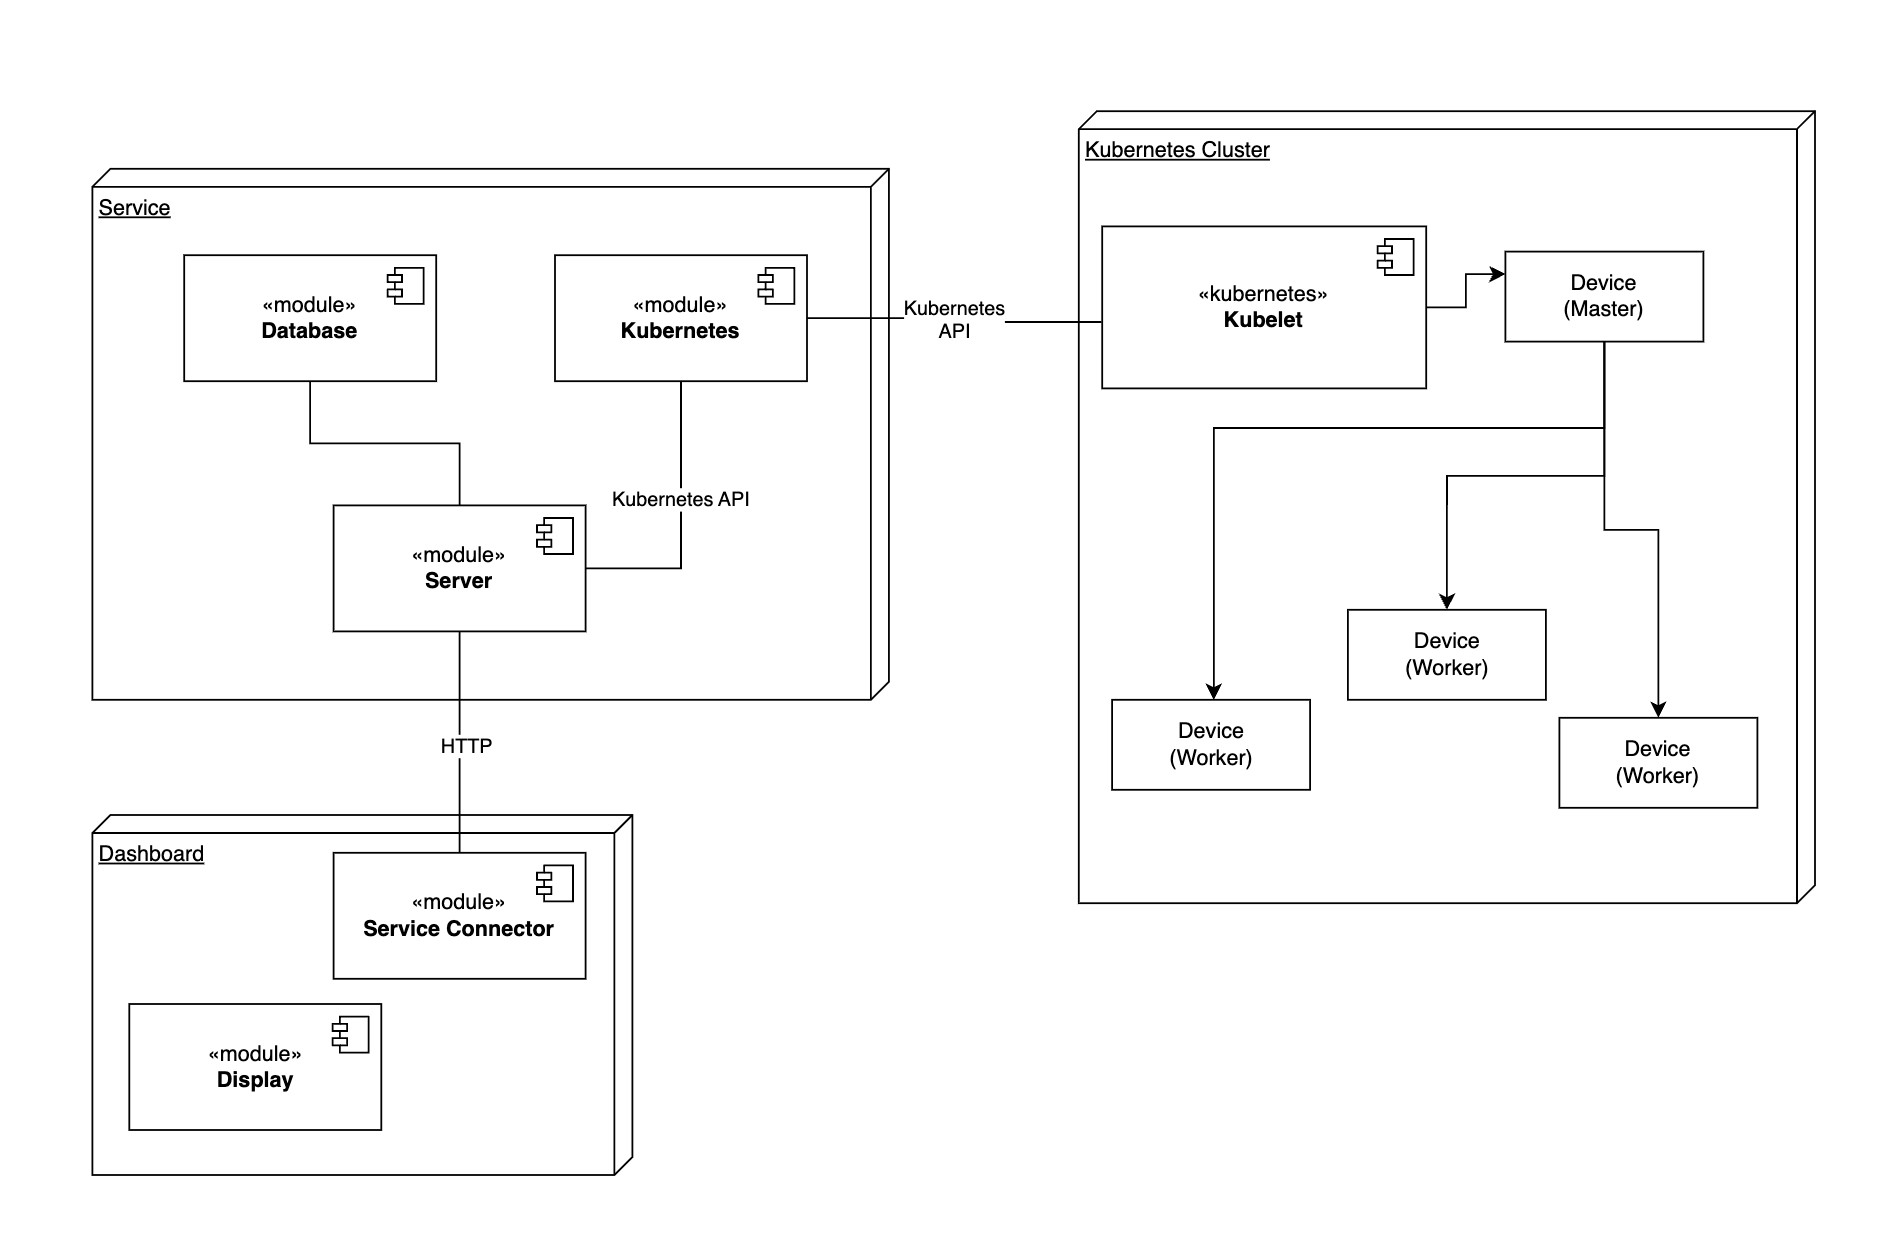
\includegraphics[width=0.9\textwidth]{resources/chapter-3/package-diagram.jpg}
  \caption{Package Diagram}
  \label{fig:package-diagram}
\end{figure}



\subsection{Rancangan Behavioural}
\label{subsec:arsitektur-behavioural}

Berdasarkan \textit{use case} diagram yang telah dibuat, terdapat 13 \textit{use case} yang memiliki alur yang berbeda. Untuk menjelaskan interaksi aktor, sistem, serta objek secara terperinci digunakan diagram \textit{sequence}. Terdapat 13 \textit{sequence} pada sistem ini, diagram ini sudah termasuk interaksi antara sistem \textit{dashboard} dan service.

\subsubsection{Alur Mendaftarkan \textit{company}}

Pada \textit{use case} ini, admin yang berperan untuk mendaftarakan \textit{company} baru yang ingin mendaftarkan ke dalam sistem. Admin dapat melakukan request melalui HTTP Client ke server. Server melakukan validasi data dan apabila telah pass, server memasukan informasi ke \textit{database}. Akhirnya, server memberikan response berupa objek dari \textit{company} yang dapat digunakan. Ilustrasi \textit{sequence diagram} dapat dilihat pada gambar \ref{fig:usecase-01}.

\begin{figure}[ht]
  \centering
  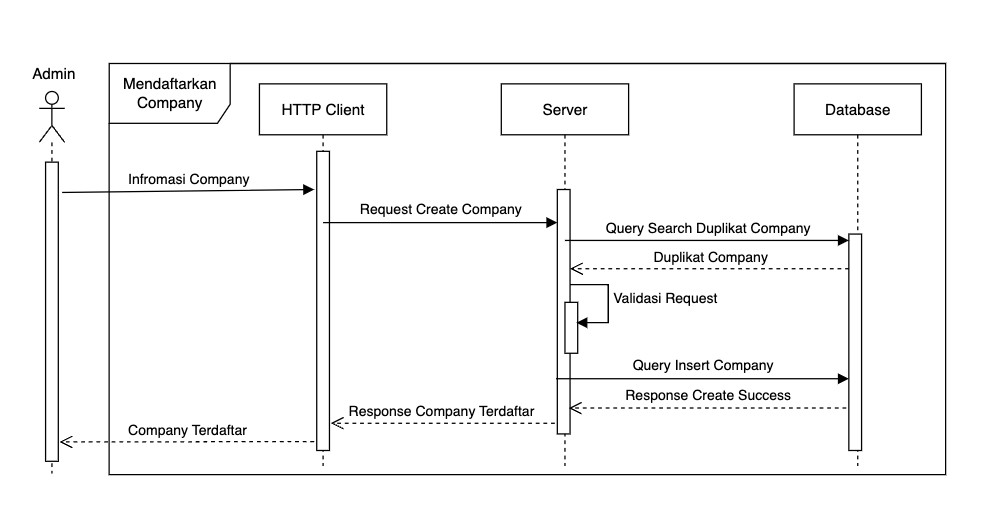
\includegraphics[width=0.7\textwidth]{resources/chapter-3/usecase/uc-01.jpg}
  \caption{\textit{Use Case} Mendaftarkan \textit{Company}}
  \label{fig:usecase-01}
\end{figure}

\subsubsection{Alur Mendaftarkan \textit{User}}

Pada \textit{use case} ini, admin yang berperan untuk mendaftarakan \textit{user} baru yang ingin mendaftarkan ke dalam sistem. Admin dapat melakukan request melalui HTTP Client ke server. Server melakukan validasi data dan apabila telah pass, server memasukan informasi ke \textit{database}. Akhirnya, server memberikan response berupa objek \textit{user} yang dapat digunakan untuk login oleh \textit{user}. Ilustrasi \textit{sequence diagram} dapat dilihat pada gambar \ref{fig:usecase-02}.

\begin{figure}[ht]
  \centering
  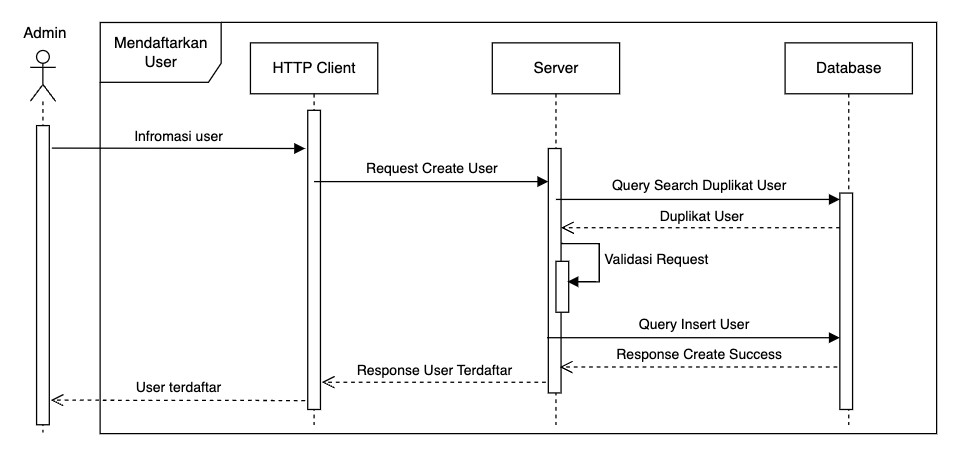
\includegraphics[width=0.8\textwidth]{resources/chapter-3/usecase/uc-02.jpg}
  \caption{\textit{Use Case} Mendaftarkan \textit{User}}
  \label{fig:usecase-02}
\end{figure}

\pagebreak

\subsubsection{Alur Manajemen \textit{company}}

Pada \textit{use case} ini, admin yang berperan untuk melakukan manajemen \textit{company}. Admin dapat menghapus ataupun mengupdate detail \textit{company}. Server melakukan validasi data, setelah melewati seluruh validasi, server melakukan update informasi yang diberikan ke \textit{database}. Server memberikan repsonse berupa hasil update. Ilustrasi \textit{sequence diagram} dapat dilihat pada gambar \ref{fig:usecase-03}.

\begin{figure}[ht]
  \centering
  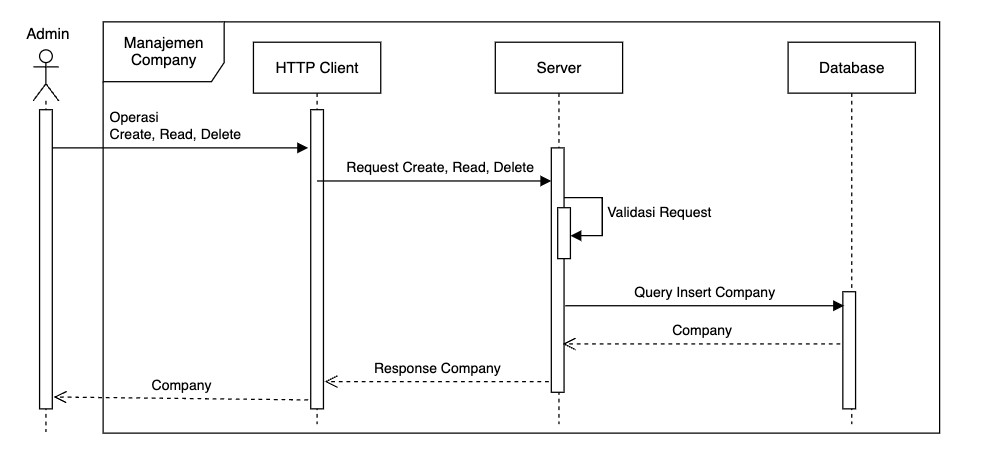
\includegraphics[width=0.8\textwidth]{resources/chapter-3/usecase/uc-03.jpg}
  \caption{\textit{Use Case} Manajemen \textit{Company}}
  \label{fig:usecase-03}
\end{figure}

\subsubsection{Alur Manajemen \textit{User}}

Pada \textit{use case} ini, admin yang berperan untuk melakukan manajemen \textit{user}. Admin dapat menghapus ataupun mengupdate detail \textit{user}. Server melakukan validasi data dan apabila telah pass, server melakukan update informasi yang diberikan ke \textit{database}. Setelah itu server memberikan repsonse berupa hasil update yang telah dilakukan. Ilustrasi \textit{sequence diagram} dapat dilihat pada gambar \ref{fig:usecase-04}.

\begin{figure}[ht]
  \centering
  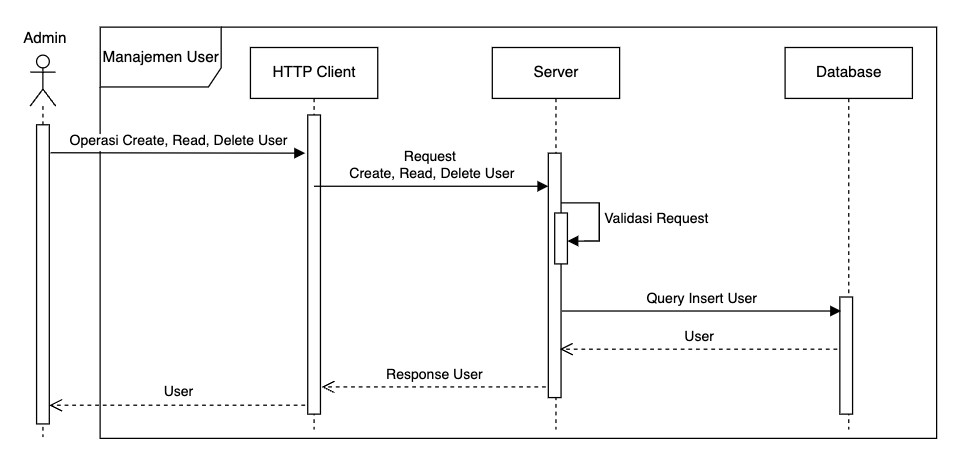
\includegraphics[width=1\textwidth]{resources/chapter-3/usecase/uc-04.jpg}
  \caption{\textit{Use Case} Manajemen \textit{User}}
  \label{fig:usecase-04}
\end{figure}

\subsubsection{Alur Login}

Pada \textit{use case} ini, \textit{user} dapat login ke dalam aplikasi dengan menginput kredensial berupa email dan password. Apabila data yang diberikan tidak valid, muncul modal untuk menandakan kesalahan yang dibuat. Apabila data benar, diberikan modal sukses lalu dilakukan \textit{redirect} ke halaman utama. Pada sisi server, terdapat beberapa validasi seperti apakah email terdapat di \textit{database} ataupun password match dengan hashed password yang ada di \textit{database}. Setelah itu, server memberikan response status ok dan memberikan \textit{user} akses ke halaman utama. Ilustrasi \textit{sequence diagram} dapat dilihat pada gambar \ref{fig:usecase-05}.

\begin{figure}[ht]
  \centering
  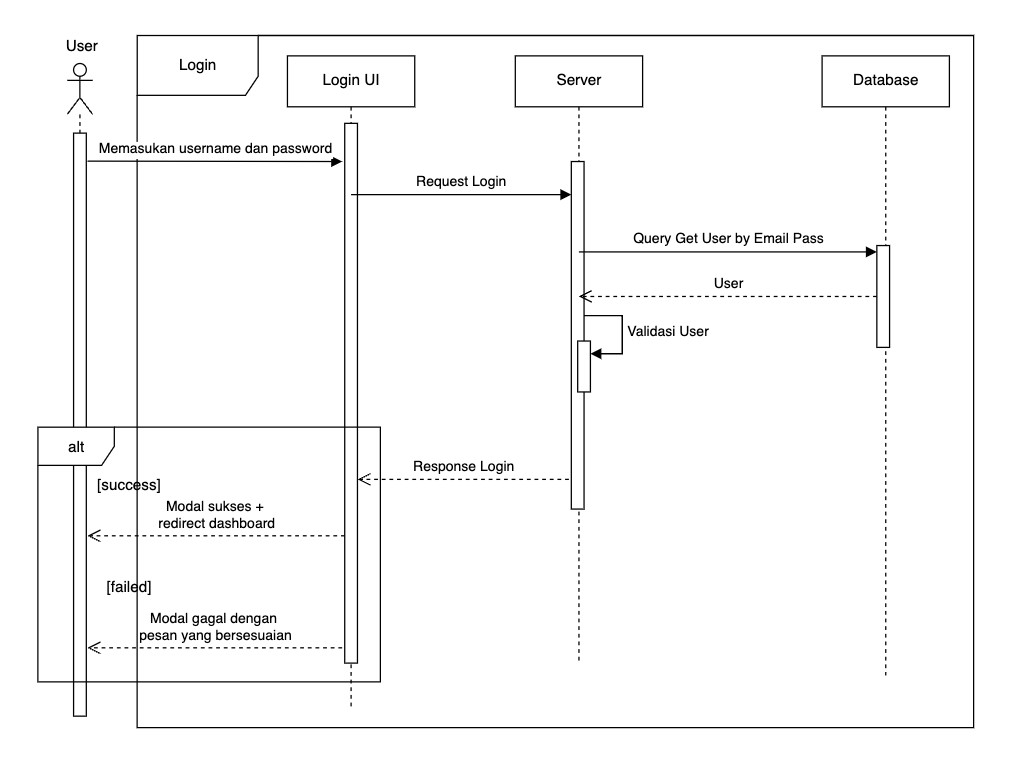
\includegraphics[width=0.8\textwidth]{resources/chapter-3/usecase/uc-05.jpg}
  \caption{\textit{Use Case} Alur Login}
  \label{fig:usecase-05}
\end{figure}

\pagebreak

\subsubsection{Alur Melihat detail \textit{company}}

Pada \textit{use case} ini, \textit{user} dapat melihat detail \textit{company} dengan cara mengunjungi halaman \textit{account}. Data diambil secara langsung melalui \textit{API Call} ke server, apabila terdapat error maka terdapat pesan error yang muncul. Apabila data berhasil di dapatkan, ditampilkan detail dari \textit{company} \textit{user}. Ilustrasi \textit{sequence diagram} dapat dilihat pada gambar \ref{fig:usecase-06}.

\begin{figure}[ht]
  \centering
  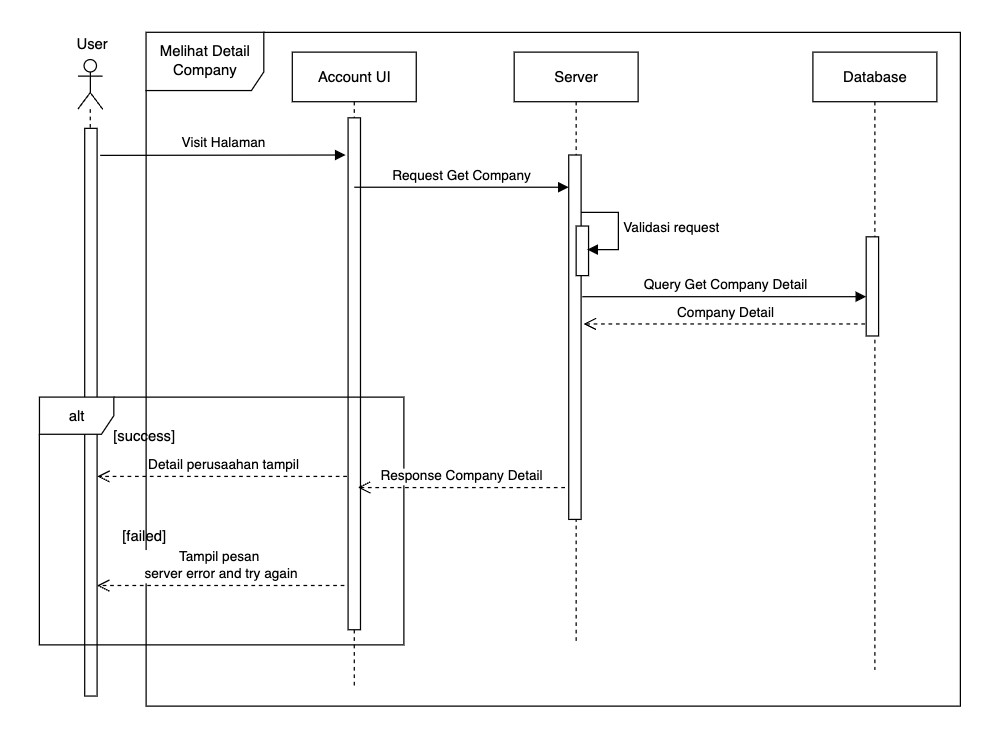
\includegraphics[width=0.8\textwidth]{resources/chapter-3/usecase/uc-06.jpg}
  \caption{\textit{Use Case} Melihat detail \textit{Company}}
  \label{fig:usecase-06}
\end{figure}

\subsubsection{Alur Melihat user lain di satu \textit{company}}

Pada \textit{use case} ini, \textit{user} dapat melihat detail seluruh user yang berada pada satu \textit{company} yang sama dengan cara mengunjungi halaman \textit{account}. Data diambil secara langsung melalui API Call ke server, apabila terdapat error maka terdapat pesan error yang muncul. Apabila data berhasil di dapatkan, ditampilkan daftar \textit{user} yang bersesuaian. Ilustrasi \textit{sequence diagram} dapat dilihat pada gambar \ref{fig:usecase-07}.


\begin{figure}[ht]
  \centering
  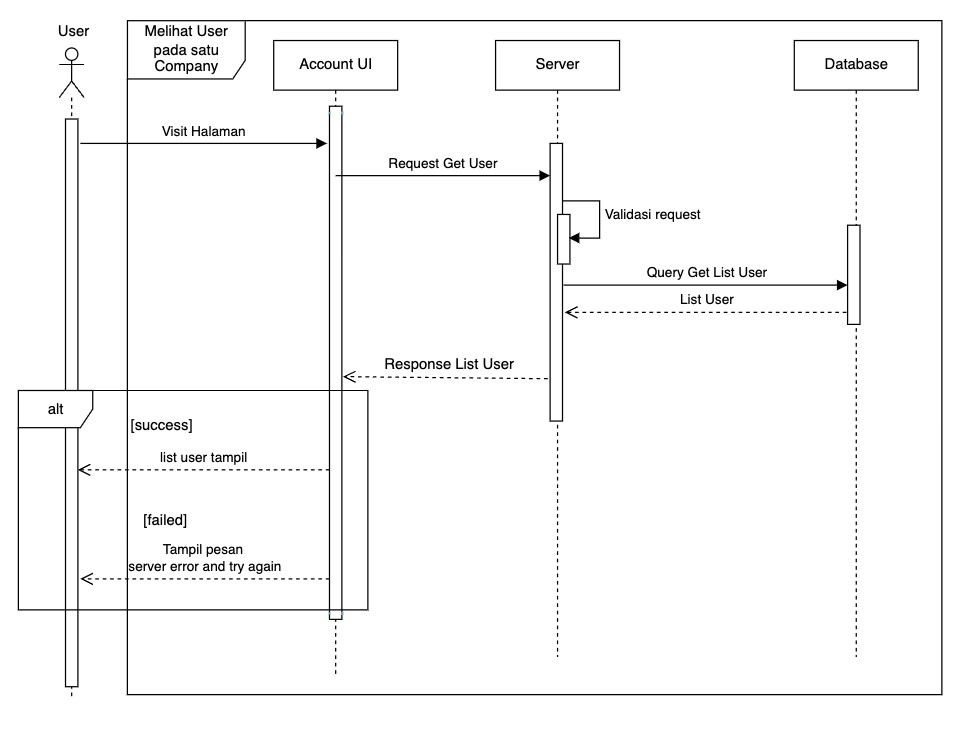
\includegraphics[width=1\textwidth]{resources/chapter-3/usecase/uc-07.jpg}
  \caption{\textit{Use Case} Melihat User Lain pada Satu \textit{Company}}
  \label{fig:usecase-07}
\end{figure}

\pagebreak

\subsubsection{Alur Manajemen \textit{Device}}

Pada \textit{use case} ini, \textit{user} dapat melakuakan manajemen \textit{device} dengan mengunjungi halaman \textit{devices}. Pada halaman ini \textit{user} dapat melakukan beberapa operasi yaitu mengambil daftar \textit{device} yang terdaftar, menambahkan \textit{device} baru, dan menghapus \textit{device}. Operasi pengambilan \textit{device} yang terdaftar dilakukan secara langsung ketika mengunjungi halaman. Operasi penghapusan ataupun penambahan \textit{device} dapat dilakukan oleh \textit{user} dengan cara menekan tombol yang ada pada laman. Ketika tombol ditekan terdapat validasi yang dilakukan pada halaman maupun pada server. Setelah melewati tahapan validasi, server melakukan update pada \textit{database}. Apabila terdapat error maka terdapat pesan error yang muncul. Apabila data berhasil di dapatkan, ditampilkan sebuah modal yang menandakan operasi berhasil untuk dilakukan. Ilustrasi \textit{sequence diagram} dapat dilihat pada gambar \ref{fig:usecase-08}.


\begin{figure}[ht]
  \centering
  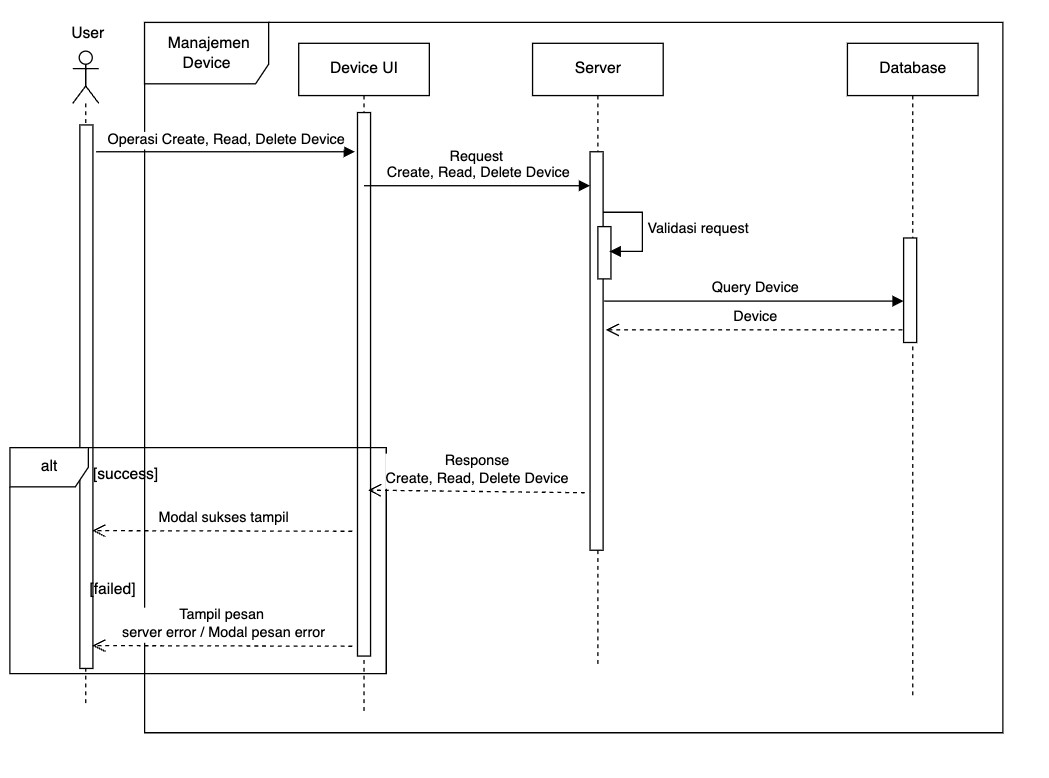
\includegraphics[width=1\textwidth]{resources/chapter-3/usecase/uc-08.jpg}
  \caption{\textit{Use Case} Manajemen \textit{Device}}
  \label{fig:usecase-08}
\end{figure}

\pagebreak

\subsubsection{Alur Manajemen \textit{Groups}}

Pada \textit{use case} ini, \textit{user} dapat melakuakan manajemen \textit{groups} dengan mengunjungi halaman \textit{groups}. Pada halaman ini \textit{user} dapat melakukan beberapa operasi yaitu mengambil daftar \textit{groups} yang terdaftar, menambahkan \textit{groups} baru, dan menghapus \textit{groups}. Operasi pengambilan \textit{groups} yang terdaftar dilakukan secara langsung ketika mengunjungi halaman. Operasi penghapusan ataupun penambahan \textit{groups} dapat dilakukan oleh \textit{user} dengan cara menekan tombol yang ada pada laman. Ketika tombol ditekan terdapat validasi yang dilakukan pada halaman maupun pada server. Setelah melewati tahapan validasi, server melakukan update pada \textit{database}. Apabila terdapat error maka terdapat pesan error yang muncul. Apabila data berhasil di dapatkan, ditampilkan sebuah modal yang menandakan operasi berhasil untuk dilakukan. Ilustrasi \textit{sequence diagram} dapat dilihat pada gambar \ref{fig:usecase-09}.


\begin{figure}[ht]
  \centering
  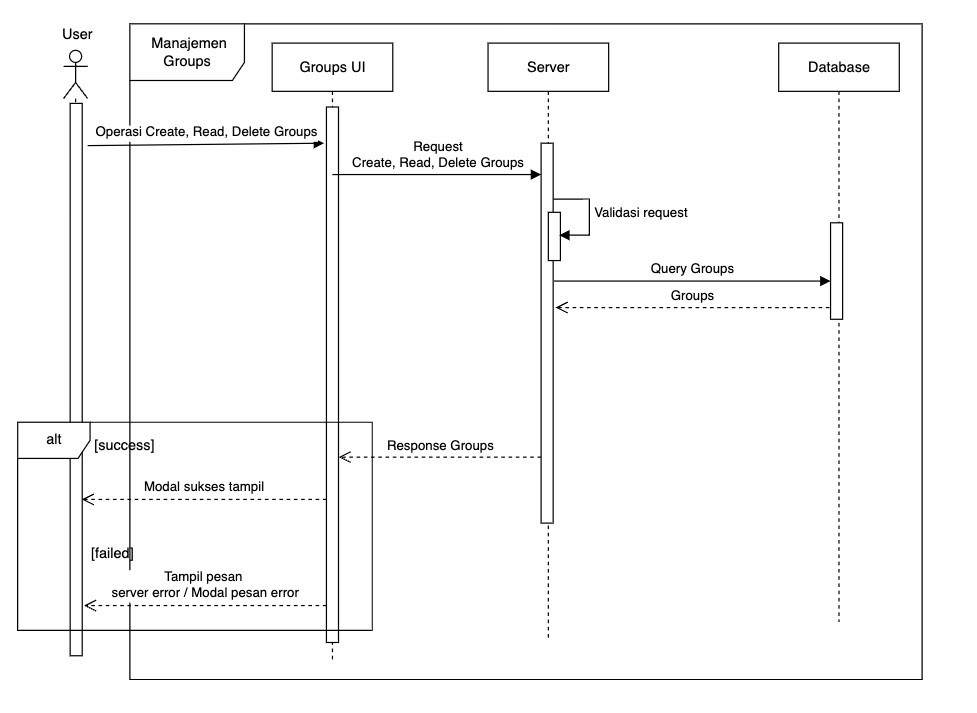
\includegraphics[width=1\textwidth]{resources/chapter-3/usecase/uc-09.jpg}
  \caption{\textit{Use Case} Manajemen \textit{Groups}}
  \label{fig:usecase-09}
\end{figure}

\pagebreak

\subsubsection{Alur Manajemen \textit{Deployment Images}}

Pada \textit{use case} ini, \textit{user} dapat melakuakan manajemen \textit{deployment images} dengan mengunjungi halaman \textit{deployments}. Pada halaman ini \textit{user} dapat melakukan beberapa operasi yaitu mengambil daftar \textit{deployment images}, menambahkan \textit{deployment images} baru, dan menghapus \textit{deployment images}. Operasi pengambilan \textit{deployment images} dilakukan secara langsung ketika membuka halaman. Operasi penghapusan ataupun penambahan \textit{deployment images} dapat dilakukan oleh \textit{user} dengan cara menekan tombol yang ada pada laman. Ketika tombol ditekan terdapat validasi yang dilakukan pada halaman maupun pada server. Setelah melewati tahapan validasi, server melakukan update pada \textit{database}. Apabila terdapat error maka terdapat pesan error yang muncul. Apabila data berhasil di dapatkan, ditampilkan sebuah modal yang menandakan operasi berhasil untuk dilakukan. Ilustrasi \textit{sequence diagram} dapat dilihat pada gambar \ref{fig:usecase-10}.

\begin{figure}[ht]
  \centering
  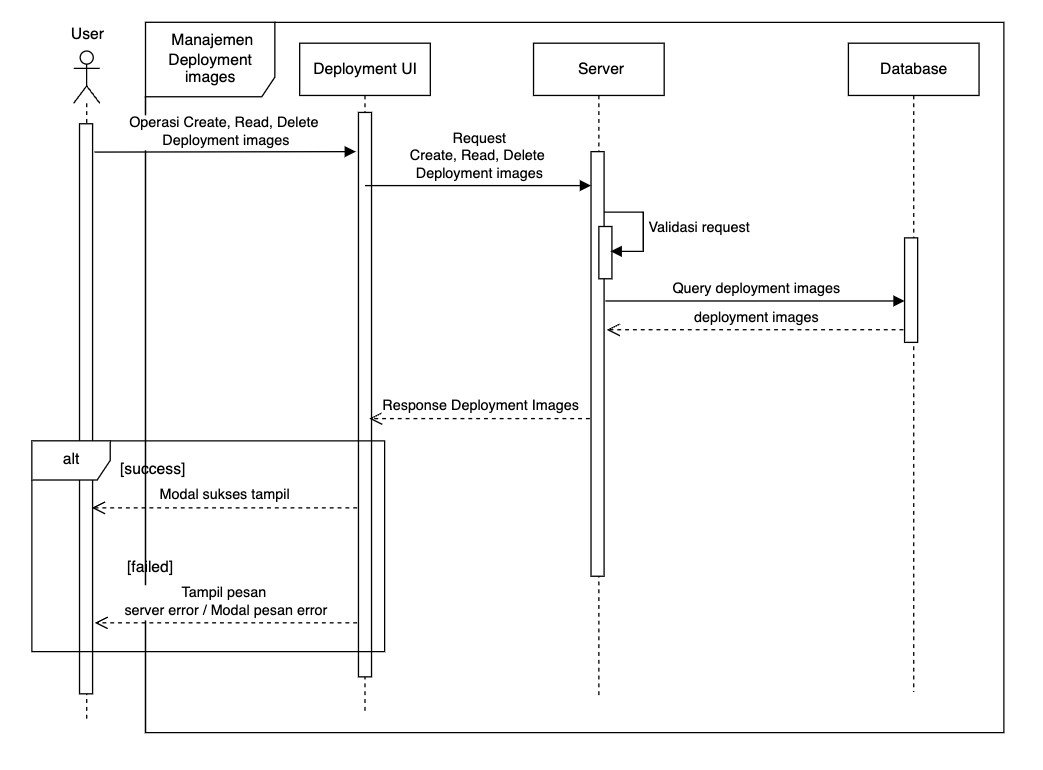
\includegraphics[width=1\textwidth]{resources/chapter-3/usecase/uc-10.jpg}
  \caption{\textit{Use Case} Manajemen \textit{Deployment Images}}
  \label{fig:usecase-10}
\end{figure}

\pagebreak

\subsubsection{Alur Manajemen \textit{Deployment Plan}}

Pada \textit{use case} ini, \textit{user} dapat melakuakan manajemen \textit{deployment plan} dengan mengunjungi halaman \textit{deployments}. Pada halaman ini \textit{user} dapat melakukan beberapa operasi yaitu mengambil daftar \textit{deployment plan} yang terdaftar, menambahkan \textit{deployment plan} baru, dan menghapus \textit{deployment plan}. Operasi pengambilan \textit{deployment plan} yang terdaftar dilakukan secara langsung ketika mengunjungi halaman. Operasi penghapusan ataupun penambahan \textit{deployment plan} dapat dilakukan oleh \textit{user} dengan cara menekan tombol yang ada pada laman. Ketika tombol ditekan terdapat validasi yang dilakukan pada halaman maupun pada server. Setelah melewati tahapan validasi, server melakukan update pada \textit{database}. Apabila terdapat error maka terdapat pesan error yang muncul. Apabila data berhasil di dapatkan, ditampilkan sebuah modal yang menandakan operasi berhasil untuk dilakukan. Ilustrasi \textit{sequence diagram} dapat dilihat pada gambar \ref{fig:usecase-11}.


\begin{figure}[ht]
  \centering
  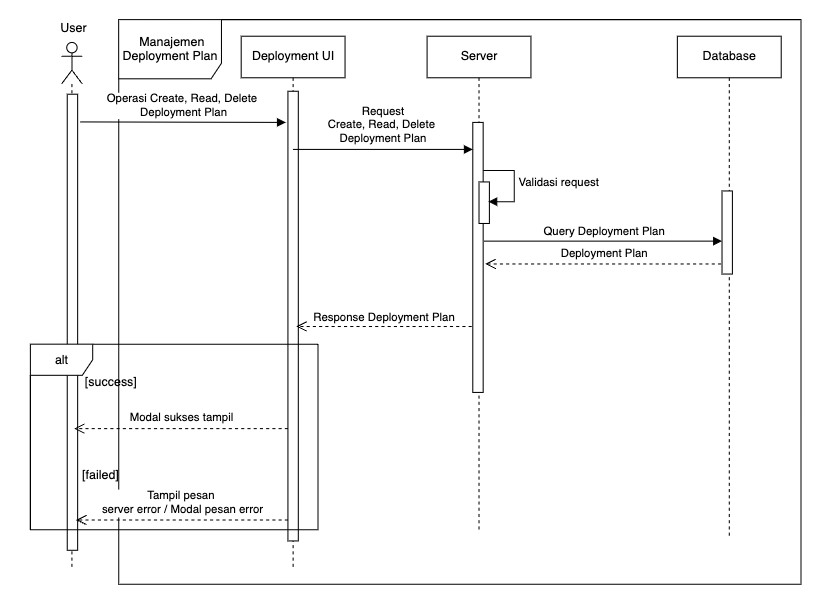
\includegraphics[width=1\textwidth]{resources/chapter-3/usecase/uc-11.jpg}
  \caption{\textit{Use Case} Manajemen \textit{Deployment Plan}}
  \label{fig:usecase-11}
\end{figure}

\pagebreak

\subsubsection{Alur \textit{remote deployment}}

Pada \textit{use case} ini, \textit{user} dapat melakukan \textit{remote deployment} dengan \textit{deployment plan} yang telah dibuat. Aksi ini dilakukan dengan cara mengunjungi halaman \textit{deployments} lalu menekan tombol deploy. Akan ada modal yang muncul memilih deployment yang dilakukan. Ketika user memilih deployment plan yang ingin di \textit{deploy}, terdapat validasi pada server sebelum melakukan deployment pada kubernetes. Setelah semua validasi berhasil dilakukan, kubernetes menginformasikan control plane pada cluster yang terhubung untuk memberikan perintah deploy kepada target. Balikan dari seluruh operasi ini adalah response berupa deployment berhasil dilakukan. Terdapat operasi \textit{asynchronus} pada \textit{background} untuk mengecek status deployment user. Ilustrasi \textit{sequence diagram} dapat dilihat pada gambar \ref{fig:usecase-12}.

\begin{figure}[ht]
  \centering
  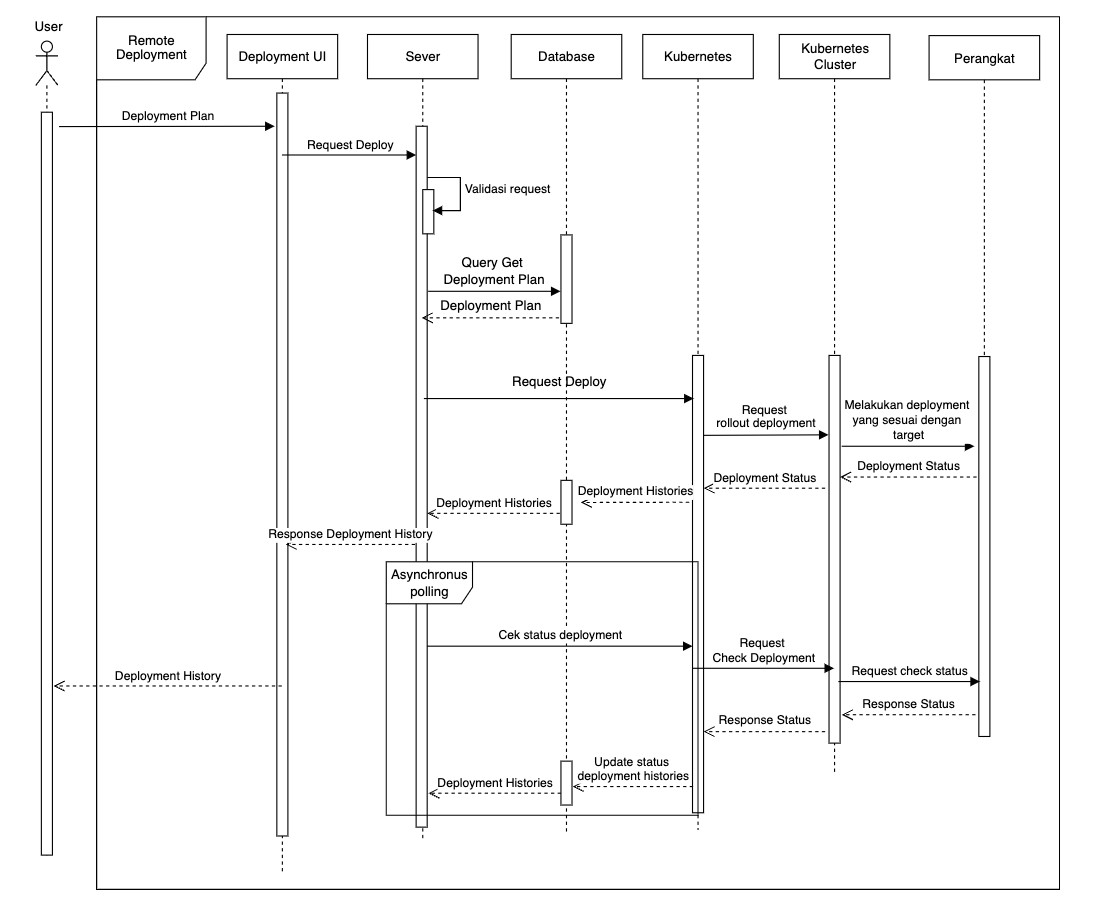
\includegraphics[width=1\textwidth]{resources/chapter-3/usecase/uc-12.jpg}
  \caption{\textit{Use Case} \textit{Remote Deployment}}
  \label{fig:usecase-12}
\end{figure}

\pagebreak

\subsubsection{Alur melihat riwayat \textit{deployment}}

Pada \textit{use case} ini, \textit{user} dapat melihat detail \textit{company} dengan cara mengunjungi halaman \textit{deployments}. Data diambil secara langsung melalui \textit{API Call} ke server, apabila terdapat error maka terdapat pesan error yang muncul. Apabila data berhasil di dapatkan, data menampilkan daftar \textit{deployment} apa saja yang telah dilakukan beserta statusnya. Ilustrasi \textit{sequence diagram} dapat dilihat pada gambar \ref{fig:usecase-13}.

\begin{figure}[ht]
  \centering
  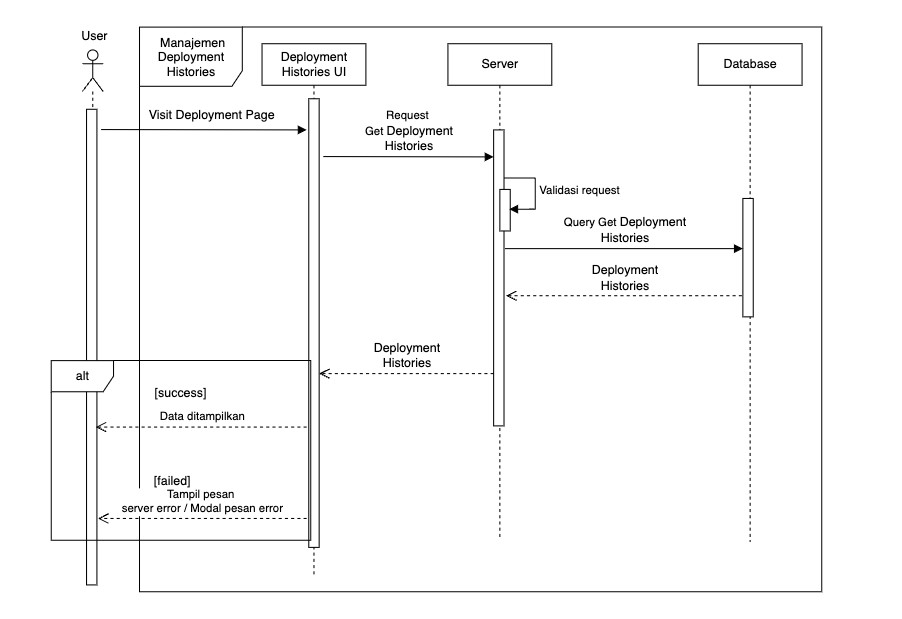
\includegraphics[width=1\textwidth]{resources/chapter-3/usecase/uc-13.jpg}
  \caption{\textit{Use Case} Melihat Riwayat \textit{Deployment}}
  \label{fig:usecase-13}
\end{figure}

\pagebreak

% \subsection{Rancangan Detail Komponen Dashboard}
\label{sec:rancangan-dashboard}

Seperti yang telah disebutkan pada bagian \ref{subsec:model-usecase} mengenai \textit{use case} diagram, bagian \ref{subsec:arsitektur-behavioural}, dan bagian \ref{subsec:arsitektur-struktural} dapat dilakukan pemetaan halaman yang dibuat untuk sistem dashboard. Terdapat dua modul yaitu modul \textit{API Connector} serta \textit{display}.

Modul \textit{API Connector} dibuat dengan cara melakukan HTTP Request ke \textit{service}. Modul display yang bertanggung jawab untuk menampilkan halaman yang digunakan oleh user. Pada modul ini terdapat 10 halaman yang dapat dilihat pada daftar di bawah ini.

\begin{enumerate}
  \item Halaman Login

        Halaman ini digunakan sebagai entrypoint dari sistem \textit{dashboard}. Pada halaman ini terdapat beberapa input yang dapat \textit{user} masukan untuk mengirimkan kredensial ke server. Setelah melalui halaman ini, barulah semua fitur dapat diakses.

  \item Halaman utama

        Halaman ini adalah halaman yang dituju oleh \textit{user} ketika telah menyelesaikan proses login. Halaman ini berisi \textit{summary} dari seluruh objek yang terdapat pada perusahaan ini.

  \item Halaman \textit{account}

        Halaman ini adalah halaman yang dapat diakses oleh \textit{user} setelah login. Halaman ini berisi informasi perusahaan \textit{user} serta daftar \textit{user} lain yang terdaftar.

  \item Halaman \textit{devices}

        Halaman ini adalah halaman yang dapat diakses oleh \textit{user} setelah login. Halaman ini berisi informasi mengenai \textit{device} apa saja yang ada pada perusahaan. \textit{user} dapat menghapus serta menambahkan \textit{device} pada halaman ini. Selain itu \textit{user} juga dapat mengunjungi laman detail dari masing masing \textit{device}.

  \item Halaman \textit{devices detail}

        Halaman ini adalah halaman yang dapat diakses oleh \textit{user} setelah login. Halaman ini dapat dituju dengan cara pergi ke halaman \textit{devices} dan memilih \textit{devices} mana yang ingin dilihat informasi lebih lanjut.


  \item Halaman \textit{groups}

        Halaman ini adalah halaman yang dapat diakses oleh \textit{user} setelah login. Halaman ini berisi informasi mengenai \textit{groups} apa saja yang ada pada perusahaan. \textit{user} dapat menghapus serta menambahkan \textit{groups} pada halaman ini. Selain itu \textit{user} juga dapat mengunjungi laman detail dari setiap \textit{groups}.

  \item Halaman \textit{groups detail}

        Halaman ini adalah halaman yang dapat diakses oleh \textit{user} setelah login. Halaman ini dapat dituju dengan cara pergi ke halaman \textit{groups} dan memilih \textit{groups} mana yang ingin dilihat informasi lebih lanjut


  \item Halaman \textit{deployments}

        Halaman ini adalah halaman yang dapat diakses oleh \textit{user} setelah login. Halaman ini berisi informasi mengenai \textit{deployment images} serta \textit{deployment plan} yang ada pada sistem. Selain itu pada halaman ini juga dapat melakukan manajemen serperti menambahkan atau menghapus baik \textit{deployment images} atauapun \textit{deployment plan}. Dari halaman ini pun, dapat diakses detail \textit{deployment images} maupun \textit{deployment plan} serta melakukan \textit{remote deployment}

  \item Halaman \textit{deployments detail}

        Halaman ini menunjukan riwayat \textit{deployment} apa saja yang telah dilakukan, statusnya serta target dari \textit{deployment}.

  \item Halaman \textit{faq}

        Halaman ini bertujuan untuk memberikan informasi mengenai tata cara hal yang perlu dilakukan sebelum mendaftarkan \textit{device} ke sistem


\end{enumerate}

% \subsection{Rancangan Detail Komponen Service}
\label{sec:rancangan-service}

Berdasarkan \textit{sequence diagram} yang telah dibuat pada bagian \ref{subsec:arsitektur-behavioural}. Sistem \textit{service} dibagi menjadi beberapa domain. Pembagian domain berfungsi untuk memfokuskan implementasi serta memudahkan tahapan testing. Terdapat 6 domain yaitu \textit{company}, \textit{user}, \textit{devices}, \textit{groups}, \textit{deployment}, dan \textit{external services}. Setiap domain memiliki diagram kelas yang menjelaskan rancangan implementasi. \textit{package} diagram dan \textit{class} diagram secara keseluruhan dapat dilihat pada gambar \ref{fig:package-diagram} dan \ref{fig:package-class-domain-diagram}.
\begin{figure}[ht]
  \centering
  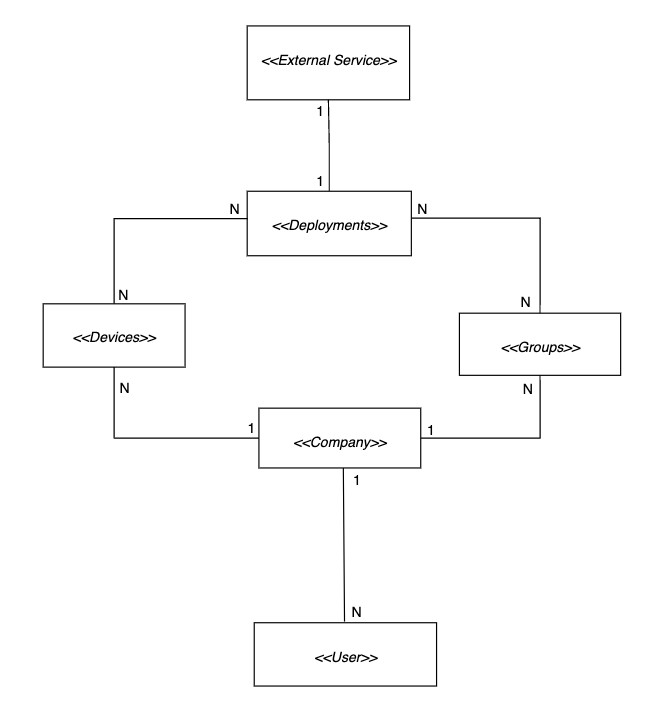
\includegraphics[width=0.6\textwidth]{resources/chapter-3/class/class-diagram-overall.jpg}
  \caption{\textit{Package Diagram Domain Service}}
  \label{fig:package-class-domain-diagram}
\end{figure}

\pagebreak

\subsubsection{Domain \textit{company}}

Domain ini mengatur konektivitas antara server dan \textit{database} dalam hal \textit{company}. Domain ini memiliki tiga lapisan yaitu \textit{handler, usecase, dan repository}. Lapisan \textit{repository} memiliki hubungan dengan \textit{database} serta terdapat lapisan \textit{handler} yang berinteraksi dengan request yang masuk. Ilustrasi \textit{class diagram} dapat dilihat pada gambar \ref{fig:company-class-diagram}.

\begin{figure}[ht]
  \centering
  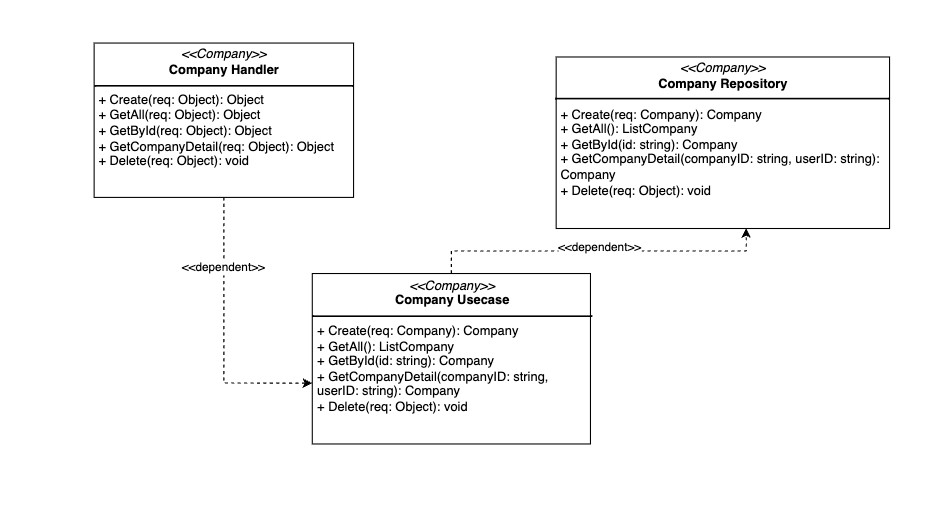
\includegraphics[width=1\textwidth]{resources/chapter-3/class/company-class-diagram.jpg}
  \caption{\textit{Company Class Diagram}}
  \label{fig:company-class-diagram}
\end{figure}

\subsubsection{Domain \textit{user}}

Domain ini mengatur konektivitas antara server dan \textit{database} dalam hal \textit{user}. Domain ini juga memliki tiga lapisan mulai dari lapisan paling luar \textit{handler}, diikuti dengan \textit{usecase} lalu terkahir \textit{repository} yang berhubungan dengan \textit{database}. Domain ini juga yang mengatur bagian autentikasi seperti login dan register. Ilustrasi \textit{class diagram} dapat dilihat pada gambar \ref{fig:user-class-diagram}.

\begin{figure}[ht]
  \centering
  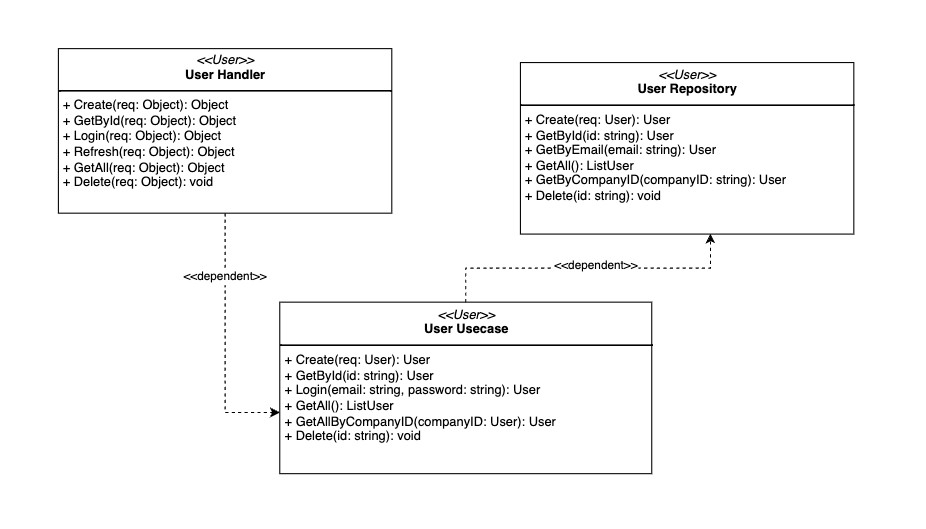
\includegraphics[width=1\textwidth]{resources/chapter-3/class/user-class-diagram.jpg}
  \caption{\textit{User Class Diagram}}
  \label{fig:user-class-diagram}
\end{figure}

\pagebreak

\subsubsection{Domain \textit{devices}}

Domain ini mengatur \textit{device} yang ada dalam sistem. Setiap \textit{device} memiliki ikatan dengan \textit{company}. Domain ini mengatur masalah CRUD dari satu \textit{company} yang dapat di \textit{manage} oleh banyak \textit{user}. Sama seperti domain lainnya, domain ini memiliki tiga lapisan yaitu \textit{handler, usecase, dan repository}. Ilustrasi \textit{class diagram} dapat dilihat pada gambar \ref{fig:device-class-diagram}.

\begin{figure}[ht]
  \centering
  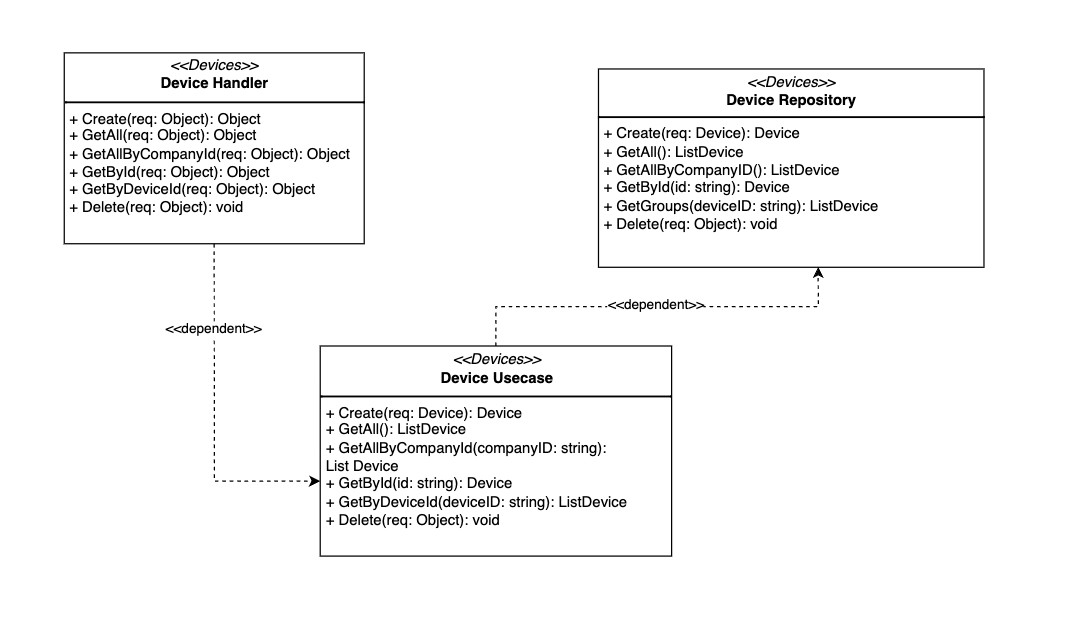
\includegraphics[width=1\textwidth]{resources/chapter-3/class/device-class-diagram.jpg}
  \caption{\textit{Device Class Diagram}}
  \label{fig:device-class-diagram}
\end{figure}

\subsubsection{Domain \textit{groups}}

Domain ini mengatur \textit{groups} yang merupakan gabungan dari satu atau lebih \textit{device}. Seperti domain \textit{devices}, domain ini pun dapat dikelompokan berdasarkan \textit{company}. Seluruh \textit{user} dapat manage \textit{groups} selama masih dalam satu perusahaan yang sama. Domain ini juga memiliki tiga lapisan yaitu \textit{handler, usecase, dan repository}. Ilustrasi \textit{class diagram} dapat dilihat pada gambar \ref{fig:groups-class-diagram}.

\begin{figure}[ht]
  \centering
  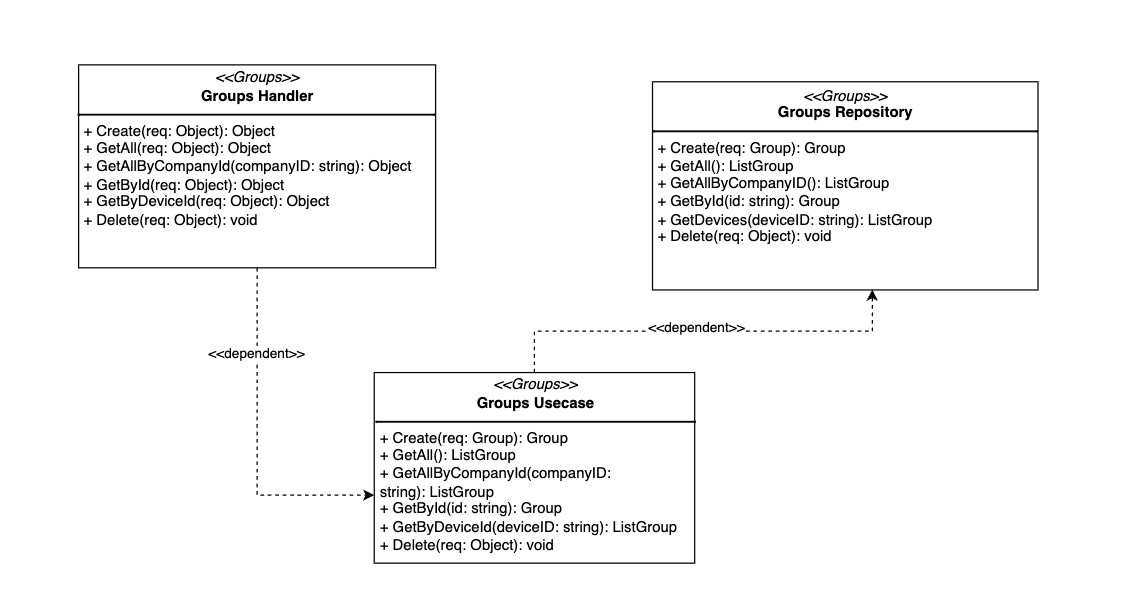
\includegraphics[width=1\textwidth]{resources/chapter-3/class/groups-class-diagram.jpg}
  \caption{Groups \textit{Class Diagram}}
  \label{fig:groups-class-diagram}
\end{figure}

\subsubsection{Domain \textit{deployment}}

Domain ini merupakan domain yang paling \textit{complex} pada service ini. Domain ini cukup luas karena berhubungan dengan \textit{deployment images} dan \textit{deployment history}. Selain itu domain ini juga memiliki hubungan dengan external service yaitu Kubernetes untuk proses deploymentnya. Ilustrasi \textit{class diagram} dapat dilihat pada gambar \ref{fig:deployment-class-diagram}.

\begin{figure}[ht]
  \centering
  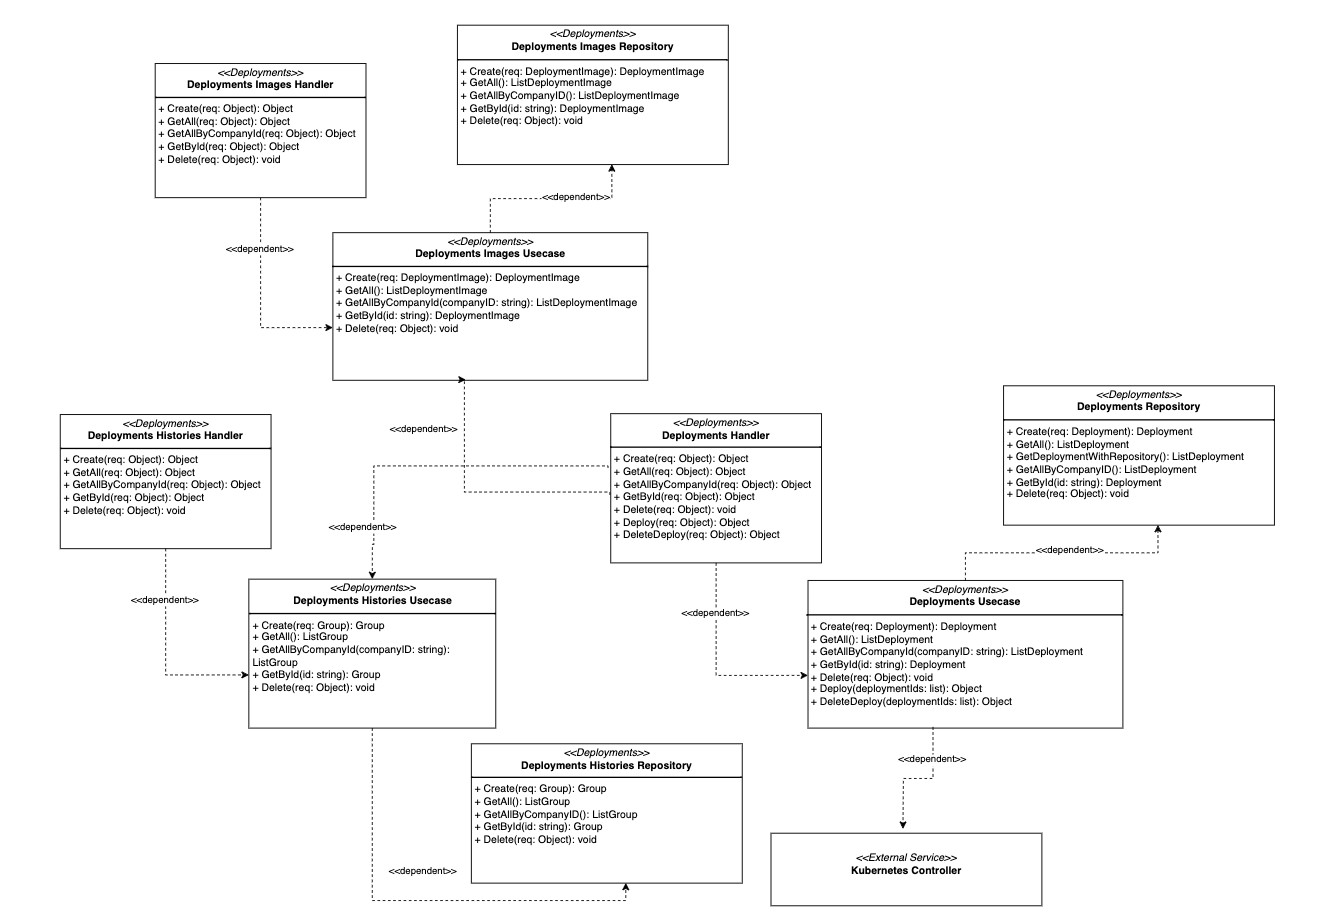
\includegraphics[width=1\textwidth]{resources/chapter-3/class/deployment-class-diagram.jpg}
  \caption{Deployment \textit{Class Diagram}}
  \label{fig:deployment-class-diagram}
\end{figure}

\pagebreak

\subsubsection{Domain \textit{external services}}

Domain ini merupakan sebuah interface dari \textit{external service} yang digunakan oleh sistem. Terdapat dua external service yaitu \textit{database} dan Kubernetes. Namun, hanya \textit{kuberntes controller} saja yang dibuat \textit{class diagram} karena untuk \textit{database} itu sudah diimplementasikan di masing masing domain pada lapisan \textit{repository}. Ilustrasi \textit{class diagram} dapat dilihat pada gambar \ref{fig:kubernetes-controller-class-diagram}.

\begin{figure}[ht]
  \centering
  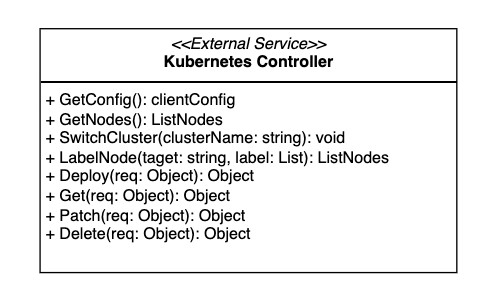
\includegraphics[width=0.7\textwidth]{resources/chapter-3/class/kubernetes-controller}
  \caption{Kubernetes Controller \textit{Class Diagram}}
  \label{fig:kubernetes-controller-class-diagram}
\end{figure}